\chapter{Implementasi dan Pengujian}

\section{Implementasi}

Bagian ini menjelaskan dari implementasi solusi yang telah dirancang sebelumnya. Bagian ini akan menjelaskan terkait lingkungan implementasi, batasan dari implementasi, serta implementasi tiap bagian dari protokol TLS.

\subsection{Batasan Implementasi}
Implementasi dilakukan dengan beberapa batasan dari protokol TLS yang telah didefinisikan pada \textcite{rfc5246}. Berikut ini merupakan batasan yang diterapkan:

\begin{enumerate}
  \item Implementasi hanya dilakukan menggunakan satdu \emph{cipher suite} saja, yaitu enkripsi menggunakan AES-256 berbasis sistem \emph{chaos}, pertukaran kunci ECDSA, algoritme hash SHA-256.
  \item Tiap pesan pada protokol \emph{handshake} dikirimkan melalui Protokol \emph{Record} yang berbeda.
  \item Fitur kompresi pada protokol TLS tidak diimplementasikan.
  \item Sertifikat digital diverifikasi secara \emph{pinning} dan tidak melakukan verifikasi \emph{revocation}.
  \item Sertifikat digital yang digunakan merupakan \emph{self-signed certificate} yang mendukung ECDSA untuk tanda tangan digital.
  \item Kurva eliptik yang didukung pada proses pertukaran kunci hanyalah kurva secp256r1.
\end{enumerate}
  
Pemilihan implementasi satu cipher ditujukan agar proses pengembangan dapat berfokus hanya pada \emph{cipher suite} yang hendak dikembangkan. Hal ini juga dapat membantu menyederhanakan pustaka yang dibangun sehingga proses pengembangan dapat lebih mudah dan cepat. 

Pemilihan pertukaran kunci berbasis ECDSA didasarkan pada kekuatan dari ECDSA. Menurut \textcite{munir2019}, ECDSA diyakini memiliki kekuatan yang setara dengan RSA walaupun dengan menggunakan kunci yang lebih pendek. Hal ini dapat membantu mengurangi \emph{resource} pada perangkat yang menggunakan pustaka ini.

Pengiriman pesan \emph{handshake} pada dasarnya dapat disatukan dalam sebuah protokol \emph{record}. Akan tetapi, pada implementasi pustaka ini, pesan \emph{handshake} dikirimkan terpisah dengan tujuan  membantu pada fase \emph{debugging} melalui aplikasi Wireshark dikarenakan tiap layer protokol \emph{record} akan ditampilkan secara terpisah.

Pada implementasi, fitur kompresi dinonaktifkan. Hal ini dikarenakan untuk melihat kualitas dari hasil enkripsi pada layer TLS. Kualitas yang dapat terlihat salah satunya terkait dengan hubungan antar blok serta keteracakan dari hasil enkripsi. Apabila plainteks dikomporesi, hasil enkripsi akan lebih mampat sehingga keteracakan akan sangat terlihat dan hilangnya hubungan antar blok.

Sertifikat digital yang digunakan pada implementasi ini merupakan sertifikat yang \emph{self-signed}. Fokus utama dari implementasi sertifikat digital hanya untuk memastikan bahwa MITM tidak terjadi. Oleh karena itu, implementasi berbentuk \emph{pinning} dan \emph{self-signed certificate} dinilai sudah cukup.

\subsection{Lingkungan Implementasi}

Lingkungan implementasi dari protokol TLS ditunjukan pada tabel \ref{tab:impl.env}.

\begin{table}[!h]
  \centering
  \caption{Lingkungan Implementasi} \label{tab:impl.env}
  \begin{tabular}{|p{3cm}|p{6cm}|}
    \hline
    Jenis Lingkungan & Nilai \\ \hline
    Sistem Operasi & Fedora Linux 40 \\ \hline
    Bahasa Pemrograman & Python 3.12.3 \\ \hline
    Kernel & Linux 6.8.9 \\ \hline
    Manager Paket & Pip 23.3.2 \\ \hline
  \end{tabular}
\end{table}

Pemilihan python sebagai bahasa pemrograman dikarenakan bahasa ini dapat mempermudah dalam proses pengujian dan pembentukan grafik. Selain itu, bahasa python memiliki pustaka cukup lengkap saat akan melakukan operasi matematika dan juga operasi kriptografi. Hal ini ditambah dengan hadirnya paket manager pip yang dapat menambah pustaka standar yang ada pada bahasa python.

Penggunaan Linux dalam lingkungan implementasi dikarenakan Linux memiliki fitur \emph{unix socket}. Hal ini dapat digunakan untuk melakukan simulasi jaringan melalui \emph{unit testing} sehingga tidak perlu membuka port untuk TCP. Hal ini dapat mencegah kegagalan akibat port TCP yang dipakai untuk \emph{unit testing} tidak bisa di-\emph{bind}.

Terdapat beberapa pustaka yang digunakan sebagai dependensi dari pustaka yang dibangun. Tabel \ref{tab:impl.lib} menyatakan daftar pustaka serta fungsi dari pustaka tersebut dalam pengembangan pustaka TLS berbasis sistem \emph{chaos}.

\begin{table}[!h]
  \centering
  \caption{Pustaka yang Digunakan} \label{tab:impl.lib}
  \begin{tabular}{|p{4cm}|p{9cm}|}
    \hline
    Nama Pustaka & Deskripsi \\ \hline
    \texttt{cryptography 42.0.5} & Pustaka ini digunakan untuk membantu dalam proses validasi tanda tangan digital dan \emph{parsing} sertifikat digital. Pustaka ini juga membantu dalam menghitung hasil Eliptic Curve Diffie-Hellman yang dilakukan pada saat \emph{Handshake} \\ \hline
    \texttt{pycryptodome 3.19.0} & Pustaka ini digunakan untuk membantu dalam melakukan proses enkripsi serta dekripsi pesan. Selain itu, pustaka ini juga membantu dalam menghitung operasi HMAC. \\ \hline
    \texttt{numpy 1.26.2} & Pustaka ini digunakan untuk membantu operasi pada array serta operasi \emph{floating-point}.\\ \hline
    \texttt{secrets} & Pustaka standard ini digunakan untuk melakukan \emph{secure comparation} dan membangkitkan nilai CSPRNG yang berasal dari sistem operasi. \\ \hline
    \texttt{socket} & Pustaka standard ini digunakan untuk melakukan komunikasi menggunakan protokol TCP.\\ \hline
  \end{tabular}
\end{table}

\subsection{Detail Implementasi}

Implementasi dilakukan dengan membentuk pustaka TLS yang mendukung protokol TLS versi 1.2. Pustaka ini dibangun dengan menggunakan bahasa pemrograman python. Pustaka ini dibangun dengan memanfaatkan beberapa pustaka yang telah disebutkan pada bagian sebelumnya. Implementasi dilakukan dengan membagi pustaka menjadi beberapa modul yang masing-masing modul memiliki tanggung jawab yang berbeda. Gambaran umum dari implementasi pustaka TLS berbasis sistem \emph{chaos} ditunjukan pada diagram komponen \ref{fig:impl.overview}.

\begin{figure}[!h]
  \centering
  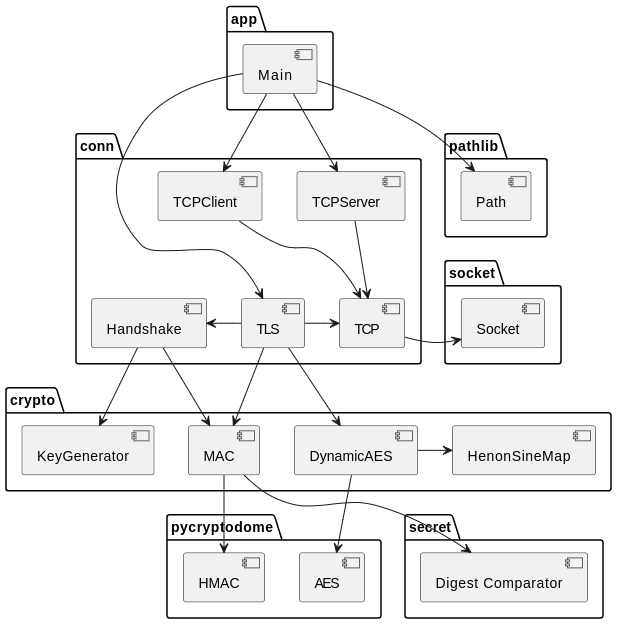
\includegraphics[width=0.9\textwidth]{chapters/res/chapter-4/impl.component.png}
  \caption{Diagram Komponen Implementasi Pustaka TLS Berbasis Sistem Chaos} \label{fig:impl.overview}
\end{figure}

Modul \texttt{main} merupakan \emph{entry point} dari aplikasi penguji dari pustaka yang dibangun. Pustaka terdiri atas beberapa modul penting, yaitu modul \texttt{data}, \texttt{conn}, dan \texttt{crypto}. Modul \texttt{data} digunakan untuk merepresentasikan data yang ada pada protokol TLS. Modul \texttt{conn} digunakan untuk mengatur komunikasi antara \emph{client} dan \emph{server}. Pada modul ini juga implementasi terkait protokol TLS dan TCP dibangun. Modul \texttt{crypto} digunakan untuk mengatur operasi kriptografi yang ada pada protokol TLS. 

Modul utilitas dan kriptografi digunakan untuk membantu dalam menyediakan fungsi-fungsi yang dapat membantu proses kriptografi, pembangkitan kunci, dan operasi lain yang dibutuhkan dalam proses pengembangan pustaka. Kelas yang ada pada modul ini dijelaskan pada tabel \ref{tab:impl.util}. Modul ini merupakan implementasi dari solusi S1, S2, S3, S4, S5, dan S6.

Tabel \ref{tab:impl.util} menjelaskan terkait fungsi utilitas yang diimplementasikan pada pustaka yang dibangun. Selain utilitas umum, terdapat beberapa kelas yang diimplementasikan sebagai utilitas yang memfasilitasi operasi kriptografi dan pembangkitan kunci acak. Tabel \ref{tab:impl.util.crypto} menjelaskan beberapa kelas yang diimplementasikan pada pustaka yang dibangun. 

Modul data digunakan untuk membantu dalam proses \emph{parsing} dan \emph{encode} data. Tabel \ref{tab:impl.data} menjelaskan beberapa kelas yang diimplementasikan pada pustaka yang dibangun. Semua kelas pada bagian ini terletak pada modul \texttt{data}. Tabel \ref{tab:impl.enum} menjelaskan beberapa enum yang diimplementasikan pada pustaka yang dibangun. Enum ini berisi beberapa konstanta yang digunakan pada protokol TLS.

Struktur data dari kelas yang diimplementasikan pada modul ini merupakan turunan dari struktur data yang didefinisikan pada \textcite{rfc5246} dan \textcite{rfc4492}. Struktur data lengkap yang menggambarkan implementasi pada penelitian ini dijelaskan pada Lampiran \ref{appendix:tls12.datatype}.

Modul \texttt{conn} bertanggung jawab dalam mengatur proses \emph{handshake}, proses komunikasi melalui TCP, komunikasi melalui UNIX Socket, serta proses enkripsi dan pengaturan \emph{state}. Tabel \ref{tab:impl.comm} menjelaskan beberapa kelas yang diimplementasikan pada pustaka yang dibangun. Semua kelas pada bagian ini terletak pada modul \texttt{conn}. Modul ini merupakan impelementasi dari solusi S3, S5, S7, S8, S9, dan S10.

\section{Pengujian}
Bagian ini menjelaskan dari pengujian yang dilakukan terhadap pustaka yang telah dibangun. Bagian ini akan menjelaskan terkait dengan detail pengujian yang dilakukan serta hasil dari pengujian tersebut.

\subsection{Tujuan Pengujian}
Pengujian dilakukan dengan tujuan sebagai berikut:
\begin{enumerate}
  \item Menguji fungsionalitas dan keamanan dari \emph{cipher} yang dibangun.
  \item Menguji fungsionalitas dan keamaman dari implementasi protokol TLS yang dibangun.
\end{enumerate}

Pengujian fungsionalitas \emph{cipher} dilakukan untuk memastikan bahwa \emph{cipher} yang dibangun dapat menjalankan proses kriptografi dengan baik. Pengujian ini dilakukan dengan melakukan operasi kriptografi pada \emph{cipher} yang telah dibangun sesuai dengan kasus yang didefinisikan. Pengujian keamanan pada \emph{cipher} dilakukan dengan melakukan uji statistik pada sistem \emph{chaos} dan \emph{cipher} yang dibangun. Hal ini bertujuan untuk mengetahui sifat statistik yang mungkin muncul pada sistem \emph{chaos} dan hasil enkripsi dari \emph{cipher} yang dibangun. Uji statistik dilakukan dengan menggunakan NIST Statistical Test Suite yang telah diimplementasikan oleh \textcite{marek2016}. Selain itu, pengujian keamanan juga dilakukan dengan menguji beberapa skenario serangan. Pengujian ini dilakukan untuk menguji jawaban atas rumusan masalah pertama.

\begin{table}[!h]
  \centering
  \caption{Lingkungan Pengujian} \label{tab:test.env}
  \begin{tabular}{|p{3cm}|p{6cm}|}
    \hline
    Jenis Lingkungan & Nilai \\ \hline
    Sistem Operasi & Fedora Linux 40 \\ \hline
    Kernel & Linux 6.8.9 \\ \hline
    Manager Paket & Pip 23.3.2 \\ \hline
    CPU & 11th Gen Intel i7-11800H (16) @ 4.600GHz \\ \hline
    RAM & 32GB \\ \hline
  \end{tabular}
\end{table}


Pengujian fungsionalitas protokol TLS dilakukan untuk memastikan bahwa protokol yang dibangun dapat berjalan dengan baik. Pengujian ini dilakukan dengan menggunakan skenario. Pengujian ini dilakukan secara \emph{end to end} testing. Pengujian keamanan protokol TLS dilakukan dengan menguji beberapa skenario serangan yang mungkin terjadi pada protokol TLS. Pengujian ini dilakukan untuk menguji jawaban atas rumusan masalah kedua.

\subsection{Lingkungan Pengujian}
Perangkat lunak dan pustaka yang digunakan pada pengujian ditunjukan pada tabel \ref{tab:test.lib}. Pengujian dilakukan pada perangkat dengan spesifikasi yang ditunjukan pada tabel \ref{tab:test.env}. 

Pengujian dilakukan pada sistem operasi linux ditujukan untuk menggunakan fitur dari \emph{UNIX socket} yang telah disediakan oleh kernel linux. Pemilihan \emph{UNIX socket} dilibatkan dalam pengujian ini dikarenakan fitur tersebut dapat mensimulasikan proses TCP tanpa perlu membuka port. Oleh karena itu, fitur ini dapat memudahkan pengujian khususnya bila menggunakan \emph{unit testing}.

\begin{table}[!h]
  \centering
  \caption{Pustaka Pengujian yang Digunakan} \label{tab:test.lib}
  \begin{tabular}{|p{4cm}|p{9cm}|}
    \hline
    Nama Pustaka & Deskripsi \\ \hline
    \texttt{pytest 8.1.1} & Pustaka ini digunakan untuk membantu dalam menyediakan \emph{runtime} pengujian dan membantu dalam proses \emph{debugging} bila terjadi kegagalan saat pengujian berlangsung. \\ \hline
    \texttt{socket} & Pustaka standard ini digunakan untuk melakukan komunikasi melalui \emph{UNIX socket}.\\ \hline
    \texttt{Fast Statictics Test v6.0.1} & Perangkat lunak ini digunakan dalam menguji keteracakan dari bytestream berdasarkan NIST Statistical Test Suite.\\ \hline
    \texttt{Wireshark} & Perangkat lunak ini digunakan dalam mengamati pesan \emph{ciphertext} yang dihasilkan oleh protokol komunikasi.\\ \hline
    \texttt{Python 3.12.3} & Perangkat lunak ini digunakan sebagai \emph{runtime} pustaka yang diuji.\\ \hline
    \end{tabular}
  \end{table}
    

  Pengujian statistik dilakukan dengan memanfaatkan Fast Statictics Test yang telah diimplementasikan oleh \textcite{marek2016}. Perangkat lunak ini merupakan optimasi dari implementasi pengujian perangkat lunak yang telah dibuat oleh NIST. Oleh karena itu, proses pengujian diharapkan dapat menjadi lebih cepat dan efisien. 

\subsection{Skenario dan Hasil Pengujian}

Bagian ini menjelaskan skenario pengujian yang dilakukan dan hasil dari pengujian yang telah disebutkan sebelumnya. Bagian ini dibagi menjadi dua bagian, yaitu pengujian \emph{cipher} dan pengujian implementasi protokol TLS.

\subsubsection{Pengujian \emph{Cipher}}

Pengujian \emph{cipher} dilakukan dengan dua tahap, yakni pengujian skenario dan pengujian statistik. Pengujian berbasis skenario dilakukan dengan beberapa skenario yang ditunjukan pada tabel \emph{test.case.cipher}. Pengujian statistik dilakukan dengan menggunakan Fast Statictics Test yang telah diimplementasikan oleh \textcite{marek2016}. Pengujian statistik ditujukan untuk menguji solusi S1 dan S4.

\begin{table}[!h]
  \centering
  \caption{Skenario Uji Cipher} \label{tab:test.case.cipher}
  \begin{tabular}{|c|p{7cm}|c|}
    \hline
    Kode Kasus Uji & Deskripsi & ID Solusi Terkait \\ \hline
    \multicolumn{3}{|l|}{Pengujian Fungsionalitas} \\ \hline
    T1.1 & \emph{Cipher} dapat melakukan proses enkripsi pada pesan teks rahasia dengan menggunakan cipher AES-256 kunci blok dinamis.  & S1, S4, dan S5\\ \hline
    T1.2 & \emph{Cipher} dapat mendekripsi kembali pesan menggunakan cipher AES-256 kunci blok dinamis. & S1, S4, dan S5\\ \hline
    \multicolumn{3}{|l|}{Pengujian Keamanan} \\ \hline
    T1.3 & Hasil dekripsi pada pesan yang dilakukan \emph{replay attack} haruslah gagal. & S1 dan S4\\ \hline
    T1.4 & Hasil enkripsi dari \emph{Cipher} pada dua blok yang memiliki pesan yang sama memiliki hasil blok yang berbeda. & S1 dan S4\\ \hline
  \end{tabular}
\end{table}

Pengujian skenario dilakukan dengan menggunakan \emph{unit testing} yang telah diimplementasikan pada pustaka yang dibangun. Pengujian ini dilakukan dengan menggunakan pustaka \texttt{pytest} yang telah dijelaskan pada bagian sebelumnya. Pengujian ini dilakukan dengan menggunakan skenario yang telah dijelaskan pada tabel \ref{tab:test.case.cipher}. Pengujian skenario dikatakan berhasil apabila semua skenario yang telah dijalankan mendapatkan hasil \emph{pass}.

Pengujian statistik pada dasarnya dilakukan dengan menguji keteracakan dari bytestream yang dihasilkan oleh sistem \emph{chaos} dan \emph{cipher}. Alasan dilakukannya pengujian keteracakan pada \emph{cipher} adalah memastikan bahwa cipher tidak memiliki pola-pola statistik yang memungkinkan melemahkan \emph{cipher} yang digunakan. Hasil dari pengujian statistik akan dibandingkan dengan acuan yang dipilih. Uji statistik ini berhasil apabila kualitas dari bytestream yang dihasilkan oleh sistem \emph{chaos} dan \emph{cipher} memiliki kualitas yang setara atau lebih baik dengan acuan yang dipilih. Kualitas ditentukan berdasarkan proporsi \emph{pass} dari uji statistik yang dilakukan. Pengujian kesetaraan dilakukan dengan uji hipotesis perbandingan proporsi dengan \emph{confidence level} sebesar 95\%.

Acuan yang digunakan untuk menilai kualitas dari keteracakan sistem \emph{chaos} adalah sistem acak \texttt{/dev/urandom} yang ada pada sistem linux. Acuan ini dipilih dikarenakan sistem acak \texttt{urandom} termasuk sistem acak aman yang sering digunakan dalam proses kriptografi. 

Acuan yang digunakan untuk menilai kualitas dari keteracakan \emph{cipher} adalah \emph{cipher} AES-256 kunci blok statis dengan blok CTR yang ada pada pustaka \texttt{pycryptodome}. Pemilihan acuan ini dikarenakan AES-256 kunci blok statis dengan blok CTR merupakan \emph{cipher} yang setara dengan implementasi \emph{cipher} yang dibangun pada penelitian ini.

Hasil dari pengujian skenario ditunjukan pada tabel \ref{tab:test.result.cipher}. Hasil tersebut menunjukan bahwa semua syarat yang dijalankan terpenuhi. Bukti serta algoritme dari pengujian ini dapat dilihat pada lampiran \ref{appendix:unit.test.cipher}. Oleh karena itu, dapat disimpulkan bahwa \emph{cipher} yang dibangun dapat berjalan dengan baik pada skenario yang telah dijalankan.

\begin{table}[!h]
  \centering
  \caption{Hasil Pengujian Cipher dengan Metode Skenario} \label{tab:test.result.cipher}
  \begin{tabular}{|c|c|}
    \hline
    Kode Kasus Uji & Hasil \\ \hline
    T1.1 & Berhasil \\ \hline
    T1.2 & Berhasil \\ \hline
    T1.3 & Berhasil \\ \hline
    T1.4 & Berhasil \\ \hline
  \end{tabular}
\end{table}

Pengujian statistik CSPRNG dilakukan dengan membandingkan proporsi \emph{pass} pada CSPRNG berbasis Sine-Henon dan CSPRNG berbasis \texttt{/dev/urandom}. Hipotesis nol ($\text{H}_0$) yang dipilih dalam pengujian ini adalah proporsi \emph{pass} dari Sine-Henon map sama dengan atau lebih besar dari proporsi \emph{pass} dari \text. Hipotesis alternatif ($\text{H}_1$) yang dipilih adalah proporsi \emph{pass} dari Sine-Henon map lebih kecil dari proporsi \emph{pass} dari \texttt{/dev/urandom}. Nilai titik kritis dari pengujian ini adalah -1.64.

\begin{table}[!h]
  \centering
  \caption{Hasil Pengujian Statistik pada CSPRNG Berbasis Sistem \emph{Chaos} Sine-Henon Map dan \texttt{/dev/urandom}} \label{tab:test.statistic.chaos}
  \begin{tabular}{|c|c|c|c|}
    \hline
    Nama Pengujian & \texttt{/dev/urandom} & Sine-Henon Map & P-Value \\ \hline
    Uji Entropi & 98,8\% & 99\% & 0,000606 \\ \hline
    Uji Frekuensi Blok & 99,2\% & 99,2\% & 0,000000 \\ \hline
    Uji Jumlah Kumulatif & 98,9\% & 99,7\% & 0,003034 \\ \hline
    Uji FFT & 98,8\% & 97,2\% & -0.003614 \\ \hline
    Uji Frekuensi & 98,4\% & 99,6\% & 0,003814 \\ \hline
    Uji Kompleksitas Linear & 98,0\% & 99,0\% & 0,002602 \\ \hline
    Uji \emph{Runs} terpanjang & 99,6\% & 98,2\% & -0,004245 \\ \hline
    Uji \emph{Non Overlapping Template} & 98,9\% & 98,2\% & -0,000193 \\ \hline
    Uji \emph{Overlapping Template} & 99,0\% & 99,0\% & 0,000000 \\ \hline
    Uji \emph{Random Excursions} & 98,6\% & 99,3\% & 0,002257 \\ \hline
    Uji \emph{Random Excursions Variant} & 98,8\% & 98,8\% & -0,000245 \\ \hline
    Uji Rank & 99,4\% & 99,4\% & 0,000000 \\ \hline
    Uji \emph{Runs} & 99,2\% & 99,2\% & 0,000000 \\ \hline
    Uji Serial & 99,3\% & 98,7\% & -0,001907 \\ \hline
    Uji Universal & 98,6\% & 99,0\% & 0,001162 \\ \hline
  \end{tabular}
\end{table}

Hasil dari pengujian statistik pada \emph{cipher} ditunjukan pada tabel \ref{tab:test.statistic.chaos}. Nilai P-value pada tabel tersebut menunjukan nilai yang lebih besar dari nilai titik kritis yang dipilih. Oleh karena itu, hipotesis nol ($\text{H}_0$) dapat diterima. Oleh karena itu, dapat disimpulkan bahwa CSPRNG berbasis sistem \emph{chaos} Sine-Henon map yang dibangun memiliki kualitas keteracakan yang setara dengan sistem random \texttt{/dev/urandom}.

Pengujian statistik pada \emph{cipher} dilakukan dengan membandingkan proporsi \emph{pass} pada \emph{cipher} berbasis AES-256 kunci blok dinamis dan \emph{cipher} berbasis AES-256 kunci blok statis dengan mode blok yang sama. Hipotesis nol ($\text{H}_0$) yang dipilih dalam pengujian ini adalah proporsi \emph{pass} dari \emph{cipher} berbasis AES-256 kunci blok dinamis sama dengan atau lebih besar dari proporsi \emph{pass} dari \emph{cipher} berbasis AES-256 kunci blok statis. Hipotesis alternatif ($\text{H}_1$) yang dipilih adalah proporsi \emph{pass} dari \emph{cipher} berbasis AES-256 kunci blok dinamis lebih kecil dari proporsi \emph{pass} dari \emph{cipher} berbasis AES-256 kunci statis. Nilai titik kritis dari pengujian ini adalah -1.64. Nilai ini diambil berdasarkan uji hipotesis perbandingan proporsi dengan \emph{confidence level} sebesar 95\%.

\begin{table}[!h]
  \centering
  \caption{Hasil Pengujian Statistik pada Cipher Blok Statis dan Blok Dinamis} \label{tab:test.statistic.cipher}
  \begin{tabular}{|c|c|c|c|}
    \hline
    Nama Pengujian & Blok Statis & Blok Dinamis & P-Value \\ \hline
    Uji Entropi & 98,6\% & 98,2\% & -0,504049 \\ \hline
    Uji Frekuensi Blok & 99,0\% & 98,4\% & 0,837512 \\ \hline
    Uji Jumlah Kumulatif & 98,5\% & 99,2\% & 1.038080 \\ \hline
    Uji FFT & 98,0\% & 98,4\% & 0,475705 \\ \hline
    Uji Frekuensi & 98,6\% & 99,2\% & 0,909550 \\ \hline
    Uji Kompleksitas Linear & 99,0\% & 99,2\% & 0,334844 \\ \hline
    Uji \emph{Runs} terpanjang & 99,2\% & 99,0\% & -0,334844 \\ \hline
    Uji \emph{Non Overlapping Template} & 99,0\% & 99,0\% & -0,037565 \\ \hline
    Uji \emph{Overlapping Template} & 99,2\% & 98,8\% & -0,635642 \\ \hline
    Uji \emph{Random Excursions} & 98,1\% & 98,6\% & -0,787570 \\ \hline
    Uji \emph{Random Excursions Variant} & 98,8\% & 99,2\% & 0,607298 \\ \hline
    Uji Rank & 99,4\% & 98,8\% & -1.004531 \\ \hline
    Uji \emph{Runs} & 98,8\% & 99,1\% & 1.674218 \\ \hline
    Uji Serial & 99,2\% & 99,0\% & 0,635642 \\ \hline
    Uji Universal & 99,4\% & 99,4\% & 0,000000 \\ \hline
  \end{tabular}
\end{table}

Hasil dari pengujian statistik pada \emph{cipher} ditunjukan pada tabel \ref{tab:test.statistic.cipher}. Nilai P-value pada tabel tersebut menunjukan nilai yang lebih besar dari nilai titik kritis yang dipilih. Oleh karena itu, hipotesis nol ($\text{H}_0$) dapat diterima. Oleh karena itu, dapat disimpulkan bahwa \emph{cipher} yang dibangun memiliki kualitas keteracakan yang setara dengan \emph{cipher} AES-256 kunci blok statis.

\subsubsection{Pengujian Implementasi Protokol TLS}

Pengujian implementasi protokol TLS dan integrasi dengan \emph{cipher} AES kunci blok dinamis dilakukan dengan pengujian skenario. Pengujian ini dilakukan secara \emph{end-to-end}. Pengujian ini dilakukan dengan tujuan untuk menguji fungsionalitas dan keamanan dari protokol TLS yang dibangun. Pengujian ini dikatakan berhasil apabila telah memenuhi semua skenario yang telah dijalankan. Skenario pengujian ditunjukan pada tabel \ref{tab:test.case.tls}.

\begin{table}[!h]
  \centering
  \caption{Skenario Uji Implementasi Protokol TLS} \label{tab:test.case.tls}
  \begin{tabular}{|c|p{7cm}|p{3cm}|}
    \hline
    Kode Kasus Uji & Deskripsi & ID Solusi Terkait \\ \hline
    \multicolumn{3}{|l|}{Pengujian Fungsionalitas} \\ \hline
    T2.1 & Protokol TLS dapat melakukan proses \emph{handshake} dan membentuk sistem \emph{chaos} yang sesuai pada tiap-tiap partisipan. & S2, S3, S7, S8, dan S9\\ \hline
    T2.2 & Protokol TLS dapat digunakan untuk mengirim dan menerima pesan teks. & S1, S4, S5, S6, dan S9 \\ \hline
    T2.3 & Protokol TLS dapat digunakan untuk mengirim dan menerima pesan biner. & S1, S4, S5, S6, dan S9 \\ \hline
    \multicolumn{3}{|l|}{Pengujian Keamanan} \\ \hline
    T2.4 & Protokol TLS dapat menangani kasus \emph{tampering} pada parameter ECDH. & S8 dan S9 \\ \hline
    T2.5 & Protokol TLS dapat menangani kasus kunci privat yang salah saat menandatangani parameter ECDH.  & S7, S8, dan S9 \\ \hline
    T2.6 & Protokol TLS dapat menangani kasus MAC yang tidak valid. & S6 dan S9 \\ \hline
    T2.7 & Protokol TLS masih dapat menerima pesan setelah mendapatkan \emph{frame} dengan MAC yang tidak valid.  & S5, S6, dan S9 \\ \hline
    T2.8 & Protokol TLS dapat menangani kasus \emph{replay attack} pada saat koneksi telah terjalin. & S5, S6, dan S9 \\ \hline
    T2.9 & Protokol TLS masih dapat menerima pesan setelah mendapatkan serangan \emph{replay}. & S5, S6, dan S9 \\ \hline
    T2.10 & Frame terenkripsi yang dihasilkan oleh protokol ini harus memiliki \emph{ciphertext} yang berbeda pada \emph{plaintext} yang sama. & S4 dan S5 \\ \hline
    T2.11 & Protokol TLS dapat menangani kasus \emph{tampering} pada pesan Client Hello. & S9 \\ \hline
    T2.12 & Protokol TLS dapat menangani kasus \emph{tampering} pada pesan Server Hello. & S9 \\ \hline
    T2.13 & Protokol TLS dapat menangani kasus \emph{certificate} server yang tidak sesuai dengan \emph{certificate pinning} pada \emph{client}.  & S9 dan S10 \\ \hline
  \end{tabular}
\end{table}


Pengujian skenario dilakukan dengan menggunakan \emph{unit testing} yang telah diimplementasikan pada pustaka yang dibangun. Pengujian ini dilakukan dengan menggunakan pustaka \texttt{pytest} yang telah dijelaskan pada bagian sebelumnya. Detail implementasi dan bukti dari pengujian ini dijelaskan pada Lampiran \ref{appendix:unit.test.tls}. Hasil pengujian skenario ditunjukan pada tabel \ref{tab:test.result.tls}

\begin{table}[!h]
  \centering
  \caption{Hasil Pengujian Implementasi TLS} \label{tab:test.result.tls}
  \begin{tabular}{|c|c|}
    \hline
    Kode Kasus Uji & Hasil \\ \hline
    T2.1 & Berhasil \\ \hline
    T2.2 & Berhasil \\ \hline
    T2.3 & Berhasil \\ \hline
    T2.4 & Berhasil \\ \hline
    T2.5 & Berhasil \\ \hline
    T2.6 & Berhasil \\ \hline
    T2.7 & Berhasil \\ \hline
    T2.8 & Berhasil \\ \hline
    T2.9 & Berhasil \\ \hline
    T2.10 & Berhasil \\ \hline
    T2.11 & Berhasil \\ \hline
    T2.12 & Berhasil \\ \hline
    T2.13 & Berhasil \\ \hline
  \end{tabular}
\end{table}

\section{Analisis Hasil Pengujian} 
\label{sec:analisis-hasil-pengujian}

Bagian ini akan membahas terkait hasil pengujian serta ancaman validitas dari hasil pengujian yang telah dilakukan. Bagian ini akan terbagi menjadi analisis hasil pengujian untuk \emph{cipher} dan analisis hasil pengujian untuk implementasi protokol TLS.

\subsection{Analisis Hasil Pengujian \emph{Cipher}}

Pengujian berbasis skenario memiliki dua kelompok pengujian. Kelompok pertama adalah pengujian fungsionalitas yang dilakukan dengan skenario T1.1 dan T1.2. Kelompok kedua adalah pengujian keamanan berbasis skenario yang dilakukan pada skenario T1.3 dan T1.4. Hasil kedua kelompok pengujian tersebut menunjukan bahwa \emph{cipher} AES blok dinamis berbasis sistem \emph{chaos} Sine-Henon map dapat bekerja dengan baik baik pada keamanan maupun fungsionalitas.

Pengujian statistik yang dilakukan pada CSPRNG menunjukan bahwa sistem random berbasis Sine-Henon map memiliki kualitas keteracakan yang setara dengan sistem random \texttt{/dev/urandom}. Selain itu, pengujian statistik yang dilakukan pada \emph{cipher} AES-256 kunci blok dinamis menunjukan bahwa \emph{cipher} yang dibangun memiliki kualitas keteracakan yang setara dengan \emph{cipher} AES-256 kunci blok statis. Oleh karena itu, kualitas keamanan dari \emph{cipher} yang dibangun dapat dikatakan setara dengan \emph{cipher} AES-256 kunci blok statis.

Berdasarkan kedua pengujian tersebut, enkripsi dengan menggunakan AES kunci blok dinamis berbasis sistem \emph{chaos} Sine-Henon map dapat digunakan sebagai \emph{cipher} yang aman dan fungsional. Metode enkripsi ini dapat digunakan dalam melakukan enkripsi pesan rahasia. Oleh karena itu, dapat disimpulkan bahwa rumusan masalah pertama dapat terjawab dengan menggunakan sistem \emph{chaos} Sine-Henon map sebagai CSPRNG penghasil kunci blok dinamis.

\subsection{Analisis Hasil Pengujian Implementasi Protokol TLS}

Pengujian implementasi protokol TLS menunjukan bahwa pengujian keamanan serta pengujian fungsionalitas dapat berjalan dengan baik. Pengujian keamanan yang dilakukan pada protokol TLS menunjukan bahwa protokol TLS yang dibangun dapat menangani \emph{replay attack}, serangan \emph{tampering}, serta serangan MITM.  Pengujian fungsionalitas yang dilakukan pada protokol TLS menunjukan bahwa protokol TLS yang dibangun dapat melakukan proses \emph{handshake}, enkripsi pesan, serta dekripsi pesan dengan baik. Oleh karena itu, dapat disimpulkan bahwa protokol TLS yang dibangun dapat digunakan sebagai protokol komunikasi yang aman dan fungsional.

Berdasarkan hasil pengujian tersebut, dapat disimpulkan bahwa \emph{cipher} AES kunci blok dinamis berbasis sistem \emph{chaos} Sine-Henon map dapat digunakan sebagai \emph{cipher} pada protokol TLS. Hal ini dikarenakan \emph{cipher} yang dibangun dapat berjalan dengan baik pada protokol TLS yang dibangun. Oleh karena itu, dapat disimpulkan bahwa rumusan masalah kedua dapat terjawab dengan menggunakan \emph{cipher} AES kunci blok dinamis berbasis sistem \emph{chaos} Sine-Henon map dengan mengikuti protokol TLSv1.2 dan penyesuaian sebagaimana yang telah dijelaskan pada bagian \ref{sec:protokol-tls-chaos}.

\subsection{Ancaman Validitas (Threat of Validity)}

Pengujian yang dilakukan memiliki beberapa ancaman validitas yang perlu diperhatikan. Hal ini dikarenakan terdapat beberapa asumsi yang diambil dalam menguji protokol ini. Asumsi yang diambil dalam pengujian ini adalah sebagai berikut:
\begin{enumerate}
  \item Pengujian mengasumsikan bahwa protokol TLS telah teruji keamanannya, sehingga serangan selain yang berkaitan dengan pembentukan \emph{cipher} dan \emph{ciphertext} tidak diuji.
  \item Pengujian mengasumsikan bahwa \emph{cipher} AES tahan terhadap serangan \emph{brute-force} dan \emph{side-channel} sehingga metode serangan tersebut tidak diuji.
  \item Proses serangan MITM diasumsikan dilakukan dengan mengganti sertifikat digital yang digunakan pada protokol TLS.
  \item Serangan \emph{tampering} hanya dilakukan pada \emph{frame} yang berkaitan dengan pembentukan \emph{cipher} dan \emph{ciphertext}. Hal ini bertujuan agar dapat mengubah atau membaca pesan yang dikirimkan.
  \item Serangan \emph{side-channel} yang dilakukan diasumsikan dilakukan dengan mengamati pola \emph{ciphertext} yang dihasilkan oleh protokol TLS.
\end{enumerate}
